\chapter{分子图学习与基于扩散模型的图生成}
\label{chap:diffusion-based_molgen}

\section{分子图学习}
在图学习中通常有两类监督任务:节点分类/回归和图分类/回归。对于图学习,一个分子可以被抽象为一个图 $\mathcal{G} = (\mathcal{V}, \mathcal{E})$,其中 $|\mathcal{V}| = n$表示节点(原子)的集合,$|\mathcal{E}| = m$ 表示分子中的边(化学键)的集合。我们用$e_i$表示节点 $i$的特征,用$e_{ij}$表示边$(i, j)$的特征。

\begin{figure}[h]
    \centering
    
\includegraphics[width=\linewidth]{figures/molecular_learning.png}
    \caption{分子学习常见泛式示意图}
    \label{fig:molecularlearning}
\end{figure} 

在节点分类或回归任务中,每个节点$i$都有一个标签或目标$y_i$。任务目标是通过学习,预测未见节点的标签。这个任务可被应用于许多应用,比如识别分子中的功能团或预测各个原子的性质。

此外,在图分类或回归任务中,给定一组图$\{ \mathcal{G}_1, \mathcal{G}_2, ..., \mathcal{G}_N \}$和对应的标签或目标 $\{ y_1, ..., y_N \}$。此时任务目标是根据图的结构和节点边的特征,预测给定图的标签或目标。这个任务被广泛应用于化合物分类或基于结构预测分子性质等。

在这两类任务中,目标是利用监督学习技术训练模型,有效地捕捉图的结构与相关标签/目标之间的关系。现有的图学习方法主要有基于图神经网络的模型和基于Transformer架构的模型。

\begin{figure}[h]
    \centering
    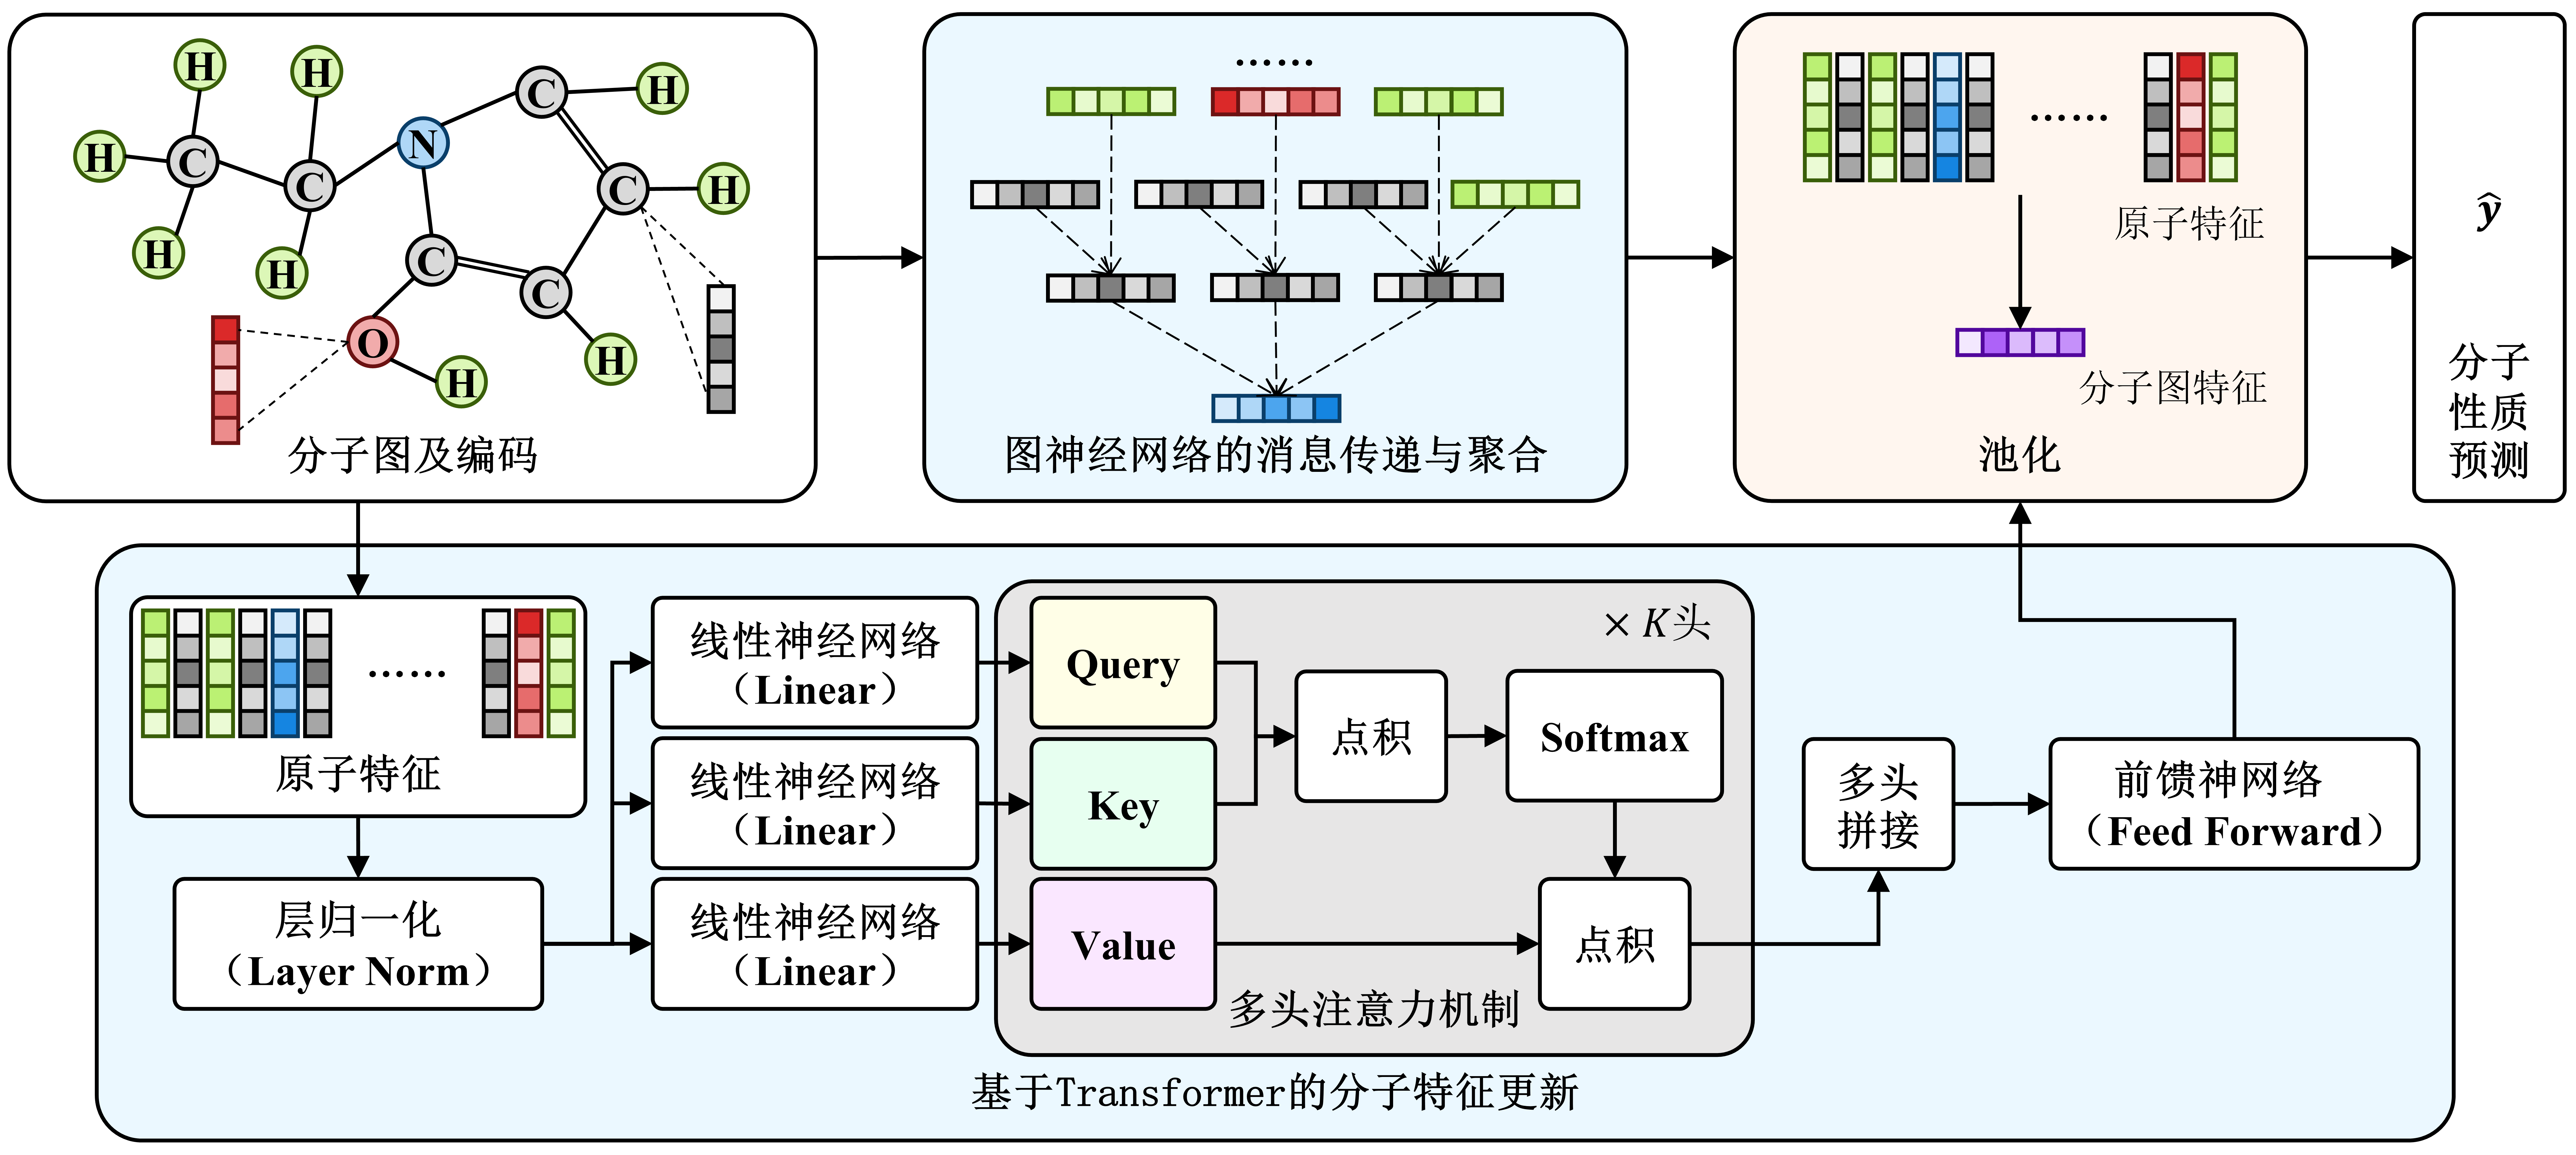
\includegraphics[width=\linewidth]{figures/gnn_transformer.png}
    \caption{基于图神经网络或Transformer的分子性质预测框架}
    \label{fig:gnntransformer}
\end{figure} 

图神经网络(Graph Neural Networks / GNNs),近来在知识图谱、社交网络和药物发现等各个领域引起了广泛的关注。GNNs的核心操作在于将图中节点或边之间的特征进行传递(也称为邻居聚合)。消息传递操作通过聚合节点$i$的邻居节点和边的隐式特征来迭代更新节点$i$自身的隐式特征$e_i$。一般来说,消息传递过程包含多轮迭代,每轮迭代可以被视为对更远距离邻居的消息聚合。假设有$L$轮迭代,第$l$轮迭代会将目标节点的l跳邻居特征注入目标节点的隐式特征。第$l$轮迭代中,消息的传递与聚合可被表示为:
\begin{eqnarray}
    &m_j^{(l)} = {\rm MSG}^{(l)}(e_j^{(l-1)}), \ j \in \mathcal{N}_i, & \\
    &e_i^{(l)} = {\rm AGG}^{(l)}(\{ m_j^{(l)}, \ j \in \mathcal{N}_i \}, \ m_i^{(l)} ), &
\end{eqnarray}
其中$m_j^{(l)}$为聚合后的消息,MSG为消息聚合函数,主流的选择包括多层感知机(MLP),可学习权重。$e_i^{(l)}$为聚合后的目标节点特征,AGG为聚合函数,主流的方式有平均值池化、最大池化和图注意力机制等。对每一次消息传递,MSG和AGG函数都可能存在可训练的参数,这些参数在每轮迭代中一般是共享的。经过$L$次消息传递与聚合后,最后一次迭代后的隐式特征被视为模型预测的节点嵌入,即$e_i^{(L)}$。最后,根据具体任务需要,运用相应的READOUT函数即可得到节点信息或是全图级别的信息。

近年来,伴随Transformer模型的出现,一些研究也开始将该架构引入图学习中。多头注意机制是Transformer的核心模块,它将多个注意力层堆叠在一起,实现并行运算。一个注意力层的核心要素一般为一组查询、键、值组成,记为$(\mathbf{Q}, \mathbf{K}, \mathbf{V})$。通过查询和键的点积,经过softmax函数归一化后即可获得注意力概率,具体可表示为:
\begin{eqnarray}
    {\rm Attention}(\mathbf{Q}, \mathbf{K}, \mathbf{V}) = {\rm softmax}(\frac{\mathbf{Q} \cdot \mathbf{K}^T}{\sqrt{d}}) \cdot \mathbf{V},
\end{eqnarray}
其中$d$为注意力头数。多头注意力机制已经在广泛的应用中证明了其优异的性能。在图学习领域,基于多头注意力机制的Transformer机制不依赖于图神经网络在每一层之间进行消息传递的范式,能够对全局信息有更全面的建模。但是相应的,与图神经网络相比,Transformer模型对算力也有更高的要求。

\section{等变性要求}
等变性是涉及到几何空间的深度学习模型需要满足的基础条件。设$T_g: X \to X$是在$g \in G$上对$X$的变换集合。我们称一个函数$\phi: X \to Y$在$g$上具有等变性,如果存在一个变换$S_g: Y \to Y$,使得下式成立:
\begin{equation}
    \phi (T_g(x)) = S_g(\phi (x))
\end{equation}

假设$\phi (\cdot)$是一个非线性函数,$x = (x_1, ..., x_N) \in \mathbb{R}^{N \times d}$是在$d$维空间中的点云输入集合,$\phi (x) = y \in \mathbb{R}^{N \times d}$是经变换后的点云集合,$T_g (x) = x + g$和$S_g(y) = y + g$分别是针对输入集合和输出集合的平移变换,如果两个变化具备等变性,那么输入和和输出也是等变的。如果变换 $\phi : X \to Y$对平移变换具有等变性,则先对输入集合进行平移$T_g(x)$,然后对其应用函数$\phi(T_g(x))$,得到的结果与先对原函数进行变换得到$y = \phi(x)$,然后对输出进行等效平移$T_g(y)$ 后的结果相同,满足方程$\phi (x+g) = \phi (x) + g$。在本工作中,我们探讨了以下三种粒子集合等变性:
\begin{itemize}
    \item 1. 平移等变性:将输入集合在$g \in \mathbb{R}^d$上进行平移,结果等价于对输出进行平移。令该变换$x + g$表示为$(x_1+g, ..., x_N + g)$,则有 $y+g = \phi (x+g)$。
    \item 2. 旋转和反射等变性:对于任意正交矩阵$Q \in \mathbb{R}^{d \times d}$,对输入做旋转或反射变化等价于对输出结果做旋转或反射变化$Qy = \phi(Qx)$。
    \item 3. 置换等变性:对输入进行置换会等效地对输出进行相同的置换。$P(y) = \phi(P(x))$,其中$P$是行索引上的一种置换。
\end{itemize}
等变性要求在高维空间内的深度学习中是一项需要满足的基本条件。对于在$n$维空间上同时满足平移,旋转,和置换不变性的变换集合,可记为E(n)。


\section{基于扩散模型的图生成}
扩散模型在生成模型中引起了相当大的关注。通过学习逆过程的去噪核,这些模型能够揭示噪声样本的潜在分布。在给定一段数据的情况下,正向过程被视为马尔可夫链,通过学习可学习参数控制噪声强度,逐渐向数据添加高斯噪声$T$次。在生成过程中,模型将噪声还原回真实数据的原始分布。
\begin{figure}[h]
    \centering
    \includegraphics[width=\linewidth]{figures/diffusion.png}
    \caption{扩散模型在计算机视觉和图生成领域的示意图}
    \label{fig:diffusion}
\end{figure} 

\subsection{扩散过程}
设$G_t (t=0, 1, ..., T)$表示分子几何信息的分布,$\beta_t \in (0, 1), t=0, 1, ..., T$表示马尔可夫链的噪声方差序列。因此我们可以得到几何信息在$t$或$T$时刻在后验分布:
\begin{eqnarray}
&q(G_{1:T} | G_0) = \prod^T_{t=1} q(G_t | G_{t-1}), & \\
&q(G_t | G_{t-1}) = \mathcal{N}(G_t; \sqrt{1-\beta_t}G_{t-1}, \beta_t I).&
\end{eqnarray}

随着时间步$t$的增加,扩散过程逐步将更多的噪声添加到原始数据分布,具体表现为噪声方差$\beta_t$从0平滑地过渡到1。设$\bar{\alpha}_t = \prod^t_{s=1} \alpha_s = \prod^t_{s=1}(1-\beta_s)$,则任意$t$时刻样本数据的分布可以表示为:
\begin{equation}
    q(G_t|G_0) = \mathcal{N}(G_t; \sqrt{\bar{\alpha}_t} G_0, (1 - \bar{\alpha}_t) I).
\end{equation} 
经过足够多的时间步$T$,初始分布被转化成白噪声,即$G_t \sim \mathcal{N}(G_t; 0, I)$。在此基础上,去噪过程会将白噪声反向还原成不带噪声的样本分布。

\subsubsection{去噪过程}
在去噪过程(也称采样过程)中,模型通过学习接近真实的逆过程$q(G_{t-1} | G_t)$的马尔可夫核函数$p_\theta(G_{0:T-1}| G_{T}) = \prod^T_{t=1} p_\theta(G_{t-1} | G_t)$来重新构建原始的几何信息。每个时间步中学习到的去噪分布为: 
\begin{equation}
  p_\theta(G_{t-1} | G_t) = \mathcal{N}(G_{t-1}; \mu_\theta(G_t, t), \sigma_t^2 I),
\end{equation}
其中$\mu_\theta(G_t, t)$是可训练的神经网络,被用于近似估计均值,$\sigma^2_t = \frac{(\beta_t - \beta_{t-1})\beta_{t-1}}{(1 - \beta_{t-1}) \beta_t}$是预定义的方差。在采样过程开始时,$p_\theta(G_T)$采样自标准高斯分布中,然后通过迭代的去噪过程逐步优化参数化的神经网络,并最终还原得到初始时刻的几何信息,即采样结果。

理论上,神经网络的目标函数采用数据的对数似然函数的变分下界形式:
\begin{eqnarray}
    &{\rm log}p(G) \geq \mathcal{L}_{base} + \sum_{t=0}^T \mathcal{L}_t,& \\
    &\mathcal{L}_{base} = -KL(q(G_T|G_0)|p(G_T)),& \\
    &\mathcal{L}_t = KL(q(G_{t-1}|G_t)|p(G_{t-1}|G_t)). &
\end{eqnarray}
然而,研究发现,神经网路预测的高斯噪声$\epsilon$能够更容易的用于训练。因此,在实际优化神经网络时,神经网路常用的目标函数$\mathcal{L}_t$ \cite{vaediff_kingma_21}形式为:
\begin{equation}
    \mathcal{L}_t = E_{\epsilon_t \sim \mathcal{N}(0, I)}[\frac{1}{2}(1- \frac{{\rm SNR}(t-1)}{{\rm SNR}(t)})||\epsilon_t - \hat{\epsilon}_t||^2].
\end{equation}

